%\documentclass[xcolor=dvipsnames,onlymath,12pt]{beamer}
\documentclass[xcolor=dvipsnames,onlymath,12pt,handout]{beamer}
\usepackage{graphics,amsmath,listings}
\usecolortheme[named=Sepia]{structure} 
%\usetheme[height=12mm]{Rochester}
\usetheme{default}
\usefonttheme{serif}

\definecolor{gray}{rgb}{0.8,0.8,0.8}
\lstset{frame=single,basicstyle=\tiny,backgroundcolor=\color{gray}}

\renewcommand{\thefootnote}{\fnsymbol{footnote}}

%\setbeamertemplate{titlepage}{\includegraphics[width=0.25\textwidth]{fsu_seal.png}}
\setbeamertemplate{blocks}[rounded][shadow=true]
\setbeamertemplate{navigation symbols}{}  % get rid of standard footer
\newcommand{\highlight}[1]{\textcolor{BrickRed}{#1}}


\title{The Big Picture}
\subtitle{MC, MCMC and the Rest of the Universe}

\author{Sachin Shanbhag}
\institute{
  Department of Scientific Computing\\
  Florida State University,\\
  Tallahassee, FL 32306.
}
\titlegraphic{\includegraphics{../../fsuseal}}
\date{}

\begin{document}

%--- the titlepage frame -------------------------%
\begin{frame}[plain]
  \titlepage
\end{frame}

\begin{frame}{The Big Picture}
\begin{center}

\includegraphics[scale=0.4]{figs/calvin_big_picture.png}
\par
credit: Bill Watterson
\end{center}

\bigskip

In this lecture, I will reveal a conceptual map to tie some things together.
\end{frame}

\begin{frame}{Preface}

In 2002-2003, I was a graduate student working on a classic fitting problem in condensed matter physics.

\medskip
\pause

Given a scatter of data $\{t_i, G_i\}$, fit a sum of decaying exponentials so that:
$$G(t) = \sum_{j=1}^{{\color{blue} M}} {\color{blue}g_j} ~ e^{-t/{\color{blue}\tau_j}},$$
with $g_j > 0$, $\tau_j > 0$.

\medskip
\pause

It turns out to be a particularly tricky problem to get right.

\medskip
\pause

I eventually began using a MCMC optimization technique called simulated annealing.

\end{frame}


\begin{frame}{Preface}

While I was researching the technique, I found out that one of my buddies in the CS department, was using a variant of the same technique to solve a ``floor-planning" problem.

\begin{center}
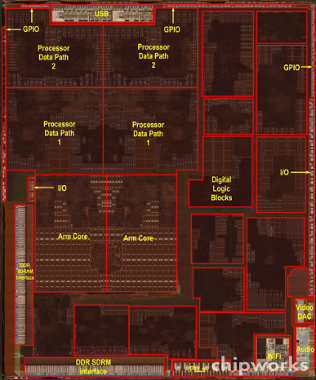
\includegraphics[scale=0.3]{figs/a5_fp}
\par
Apple A5 chip. credit: chipworks
\end{center}


\end{frame}

\begin{frame}{Preface}

\begin{columns}
  \begin{column}{0.5\textwidth}
	\begin{center}
	  
\includegraphics[scale=0.23]{figs/news.png}
	  \par
	  graphicriver.net
	\end{center}
  \end{column}
  \begin{column}{0.5\textwidth}
  Fitting chips on a substrate is closely related to a problem that newspapers have to solve everyday.

\pause
\medskip

    Laying out ``panels" of news stories.
    
    \pause
    \medskip
    
\begin{quote}
It's amazing that the amount of news that happens in the world every day always just exactly fits the newspaper. - Sienfeld
\end{quote}
  \end{column}
\end{columns}


\end{frame}

\begin{frame}{Motivation}

Monte Carlo means different things to different disciplines.

\pause
\medskip

People often use similar techniques to solve problems, which seem unique (to the people solving the problems).

\pause
\medskip

The history of MC methods is littered with nearly identical methods being  ``rediscovered" in each disciplinary silo.

\pause
\medskip

We will meet some of these methods in this class. Often, they will have multiple aliases.

\pause
\medskip

A big-picture understanding allows us to look beyond at broad themes, beyond these domain-specific boundaries.


\end{frame}

\begin{frame}{Motivation}

What is the connection between:
\begin{itemize}
\item Monte Carlo
\pause
\item Markov Chain Monte Carlo
\pause
\item Other numerical methods like finite elements, steepest descent, Gauss quadrature etc.?
\end{itemize}

\medskip
\pause

At its very core MC/MCMC can be thought of as a \highlight{sampling} technique.
\pause

\medskip

It draws or samples $x$ from any desired distribution $\pi(x)$.
\pause

\medskip

$x$ is usually multidimensional; but we will start with 1D
\pause
\medskip

Everything else flows from this simple fact.

\end{frame}

\begin{frame}{The Big Picture}

\highlight{Sampling}, by itself, is a fundamental problem.
$$x \sim \pi(x).$$

\pause

Three important sub-classes of problems are:

\pause

\begin{itemize}
\item \highlight{Integration}
$$I = \int g(x) dx,$$
\pause
or, as happens quite frequently in practice,
$$I = \int f(x) \pi(x) dx.$$
where the $\pi(x)$ highlights the relationship to the sampling problem.
\end{itemize}
\end{frame}

\begin{frame}{The Big Picture}
\begin{itemize}
\item \highlight{Optimization}
$$x^{*} = \max_{x} f(x),$$
where $x^{*}$ is the value at which $f(x)$ is maximized.

\pause
\medskip

\item \highlight{Simulation}

\medskip

This is a general term, which defines the evolution of a system subject to a particular stochastic mathematical model or rules.

\pause
\medskip

\pause
Kinetic or dynamic Monte Carlo can be used to study such problems.

\medskip
\pause
Ex: traffic modeling 

\end{itemize}

\end{frame}


\begin{frame}{The Big Picture}
\begin{center}
	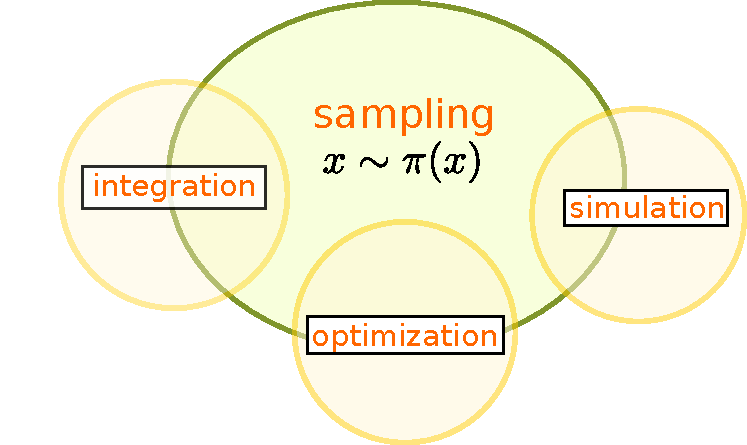
\includegraphics[scale=0.8]{figs/bigpic}

\medskip
	
	MC $\equiv$ sampling
\end{center}
\end{frame}


\begin{frame}{Interpretation}

A certain subclass of problems, say integration, can be attacked using MC or non-MC methods.

\medskip
\pause

Examples of \highlight{non-MC methods} the three sub-classes include:

\begin{itemize}
\item \highlight{Integration}

analytical, Gauss quadrature, Newton-Cotes, Clenshaw-Curtis etc.

\pause

\item \highlight{Optimization}

analytical, steepest descent, conjugate-gradient, linear-programming, Levenberg-Marquardt etc.

\pause

\item \highlight{Simulation}

analytical, finite elements, finite differences, molecular dynamics, etc.

\end{itemize}

\end{frame}

\begin{frame}{Sampling}
Prefer direct Monte Carlo, whenever possible.

\pause
\medskip

\textit{Advantage}: individual samples are \highlight{independent}, which makes error analysis easier

\pause
\medskip

But many complex problems cannot be tacked with direct MC, and MCMC becomes the method of last resort

\pause
\medskip

Samples in MCMC are \highlight{correlated}. This complicates analysis.

\pause
\medskip

\highlight{Possibly helpful analogy}:

\begin{center}
analytical : numerical :: MC : MCMC
\end{center}

In numerical solutions, we have to worry about tolerance, stability, round-off error, convergence, choice of method etc, as the price for being able to solve a wider range of problems. 

\end{frame}

%\begin{frame}{Sampling: Applications}
%Perhaps the most famous application of sampling is Bayesian inference:
%
%$$\pi(x | d) = \dfrac{\pi(d | x)\pi(x)}{\int \pi(d | x)\pi(x) dx}$$
%
%We will look at concrete examples later.
%
%\medskip
%
%Right now, note that the typical problem requires us to sample from $x \sim \pi(x | d)$
%
%\end{frame}

\end{document}
